\documentclass[letterpaper]{report}

\usepackage{calc,amsmath,amssymb,amsfonts}
\usepackage[T1]{fontenc}
\usepackage[english]{babel}
\usepackage{xcolor}
\usepackage[top=2cm,bottom=1.27cm,left=3cm,right=2cm,includefoot]{geometry}
\usepackage[style=numeric,backend=biber]{biblatex}
\usepackage{array,supertabular,hhline,hyperref}
\usepackage[pdftex]{graphicx}
\usepackage[final]{pdfpages}
% \usepackage{csquotes}

% this package best loaded last in the preamble
\usepackage{subfiles} 

\hypersetup{colorlinks=true,allcolors=blue,pdftitle=AIMS,pdfauthor=Bui Hoang Tu 20200547}
\setlength\tabcolsep{1mm}
\renewcommand\arraystretch{1.3}
\title{AIMS}
\author{Bui Hoang Tu 20200547}
\date{2023-10-15}

\begin{document}%%%%%%%%%%%%%%%%%%%%%%%%%%%%%%%%%%%%%%%%%%%%%%%%%%%%%%%%%%%%%%%%%%%%%%%%%%%%%%%%%%%%%%%%%%%%%%%%%%%%%%%

\includepdf[pages=-]{UseCaseSpecification-img/firstpage.pdf}
\setcounter{tocdepth}{3}

\tableofcontents
\clearpage

\chapter{Introduction}
\section{Objective}
This document presents the detailed description for User management subsystem, user group and their usable function at run time. This document also describes the objectives and features of the system, interfaces and constraints of the system in response to external action.
This document is for stakeholders and related software developers.

\section{Scope}
\section{Glossary}
\section{References}

\chapter{Overall requirements}
\section{Actors}
\begin{itemize}
    \item Admin: Staffs who manage the store
    \item User: Clients who use buy the products
    \item VNPay: Paying port
\end{itemize}
\clearpage

\section{General use case diagram}
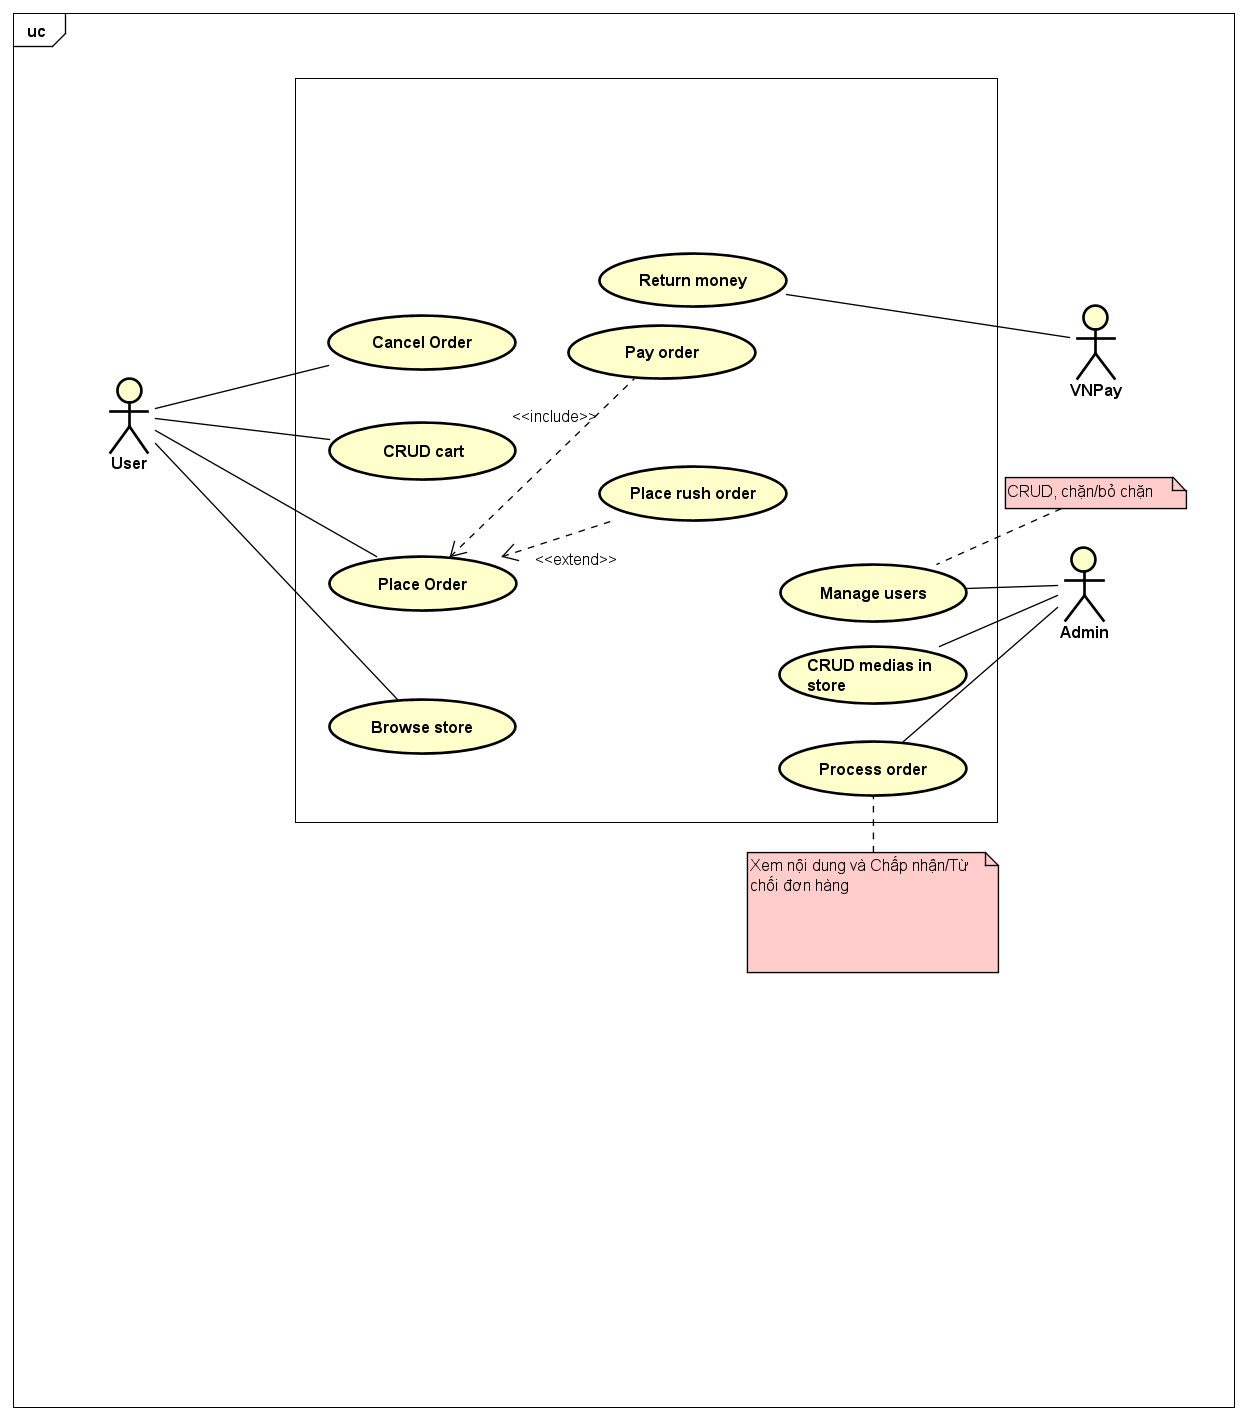
\includegraphics[width=15.24cm,height=17.353cm]{UseCaseDiagram/UseCase.png}

\section{Business processes \ \ \ \ \ \ \ \ }
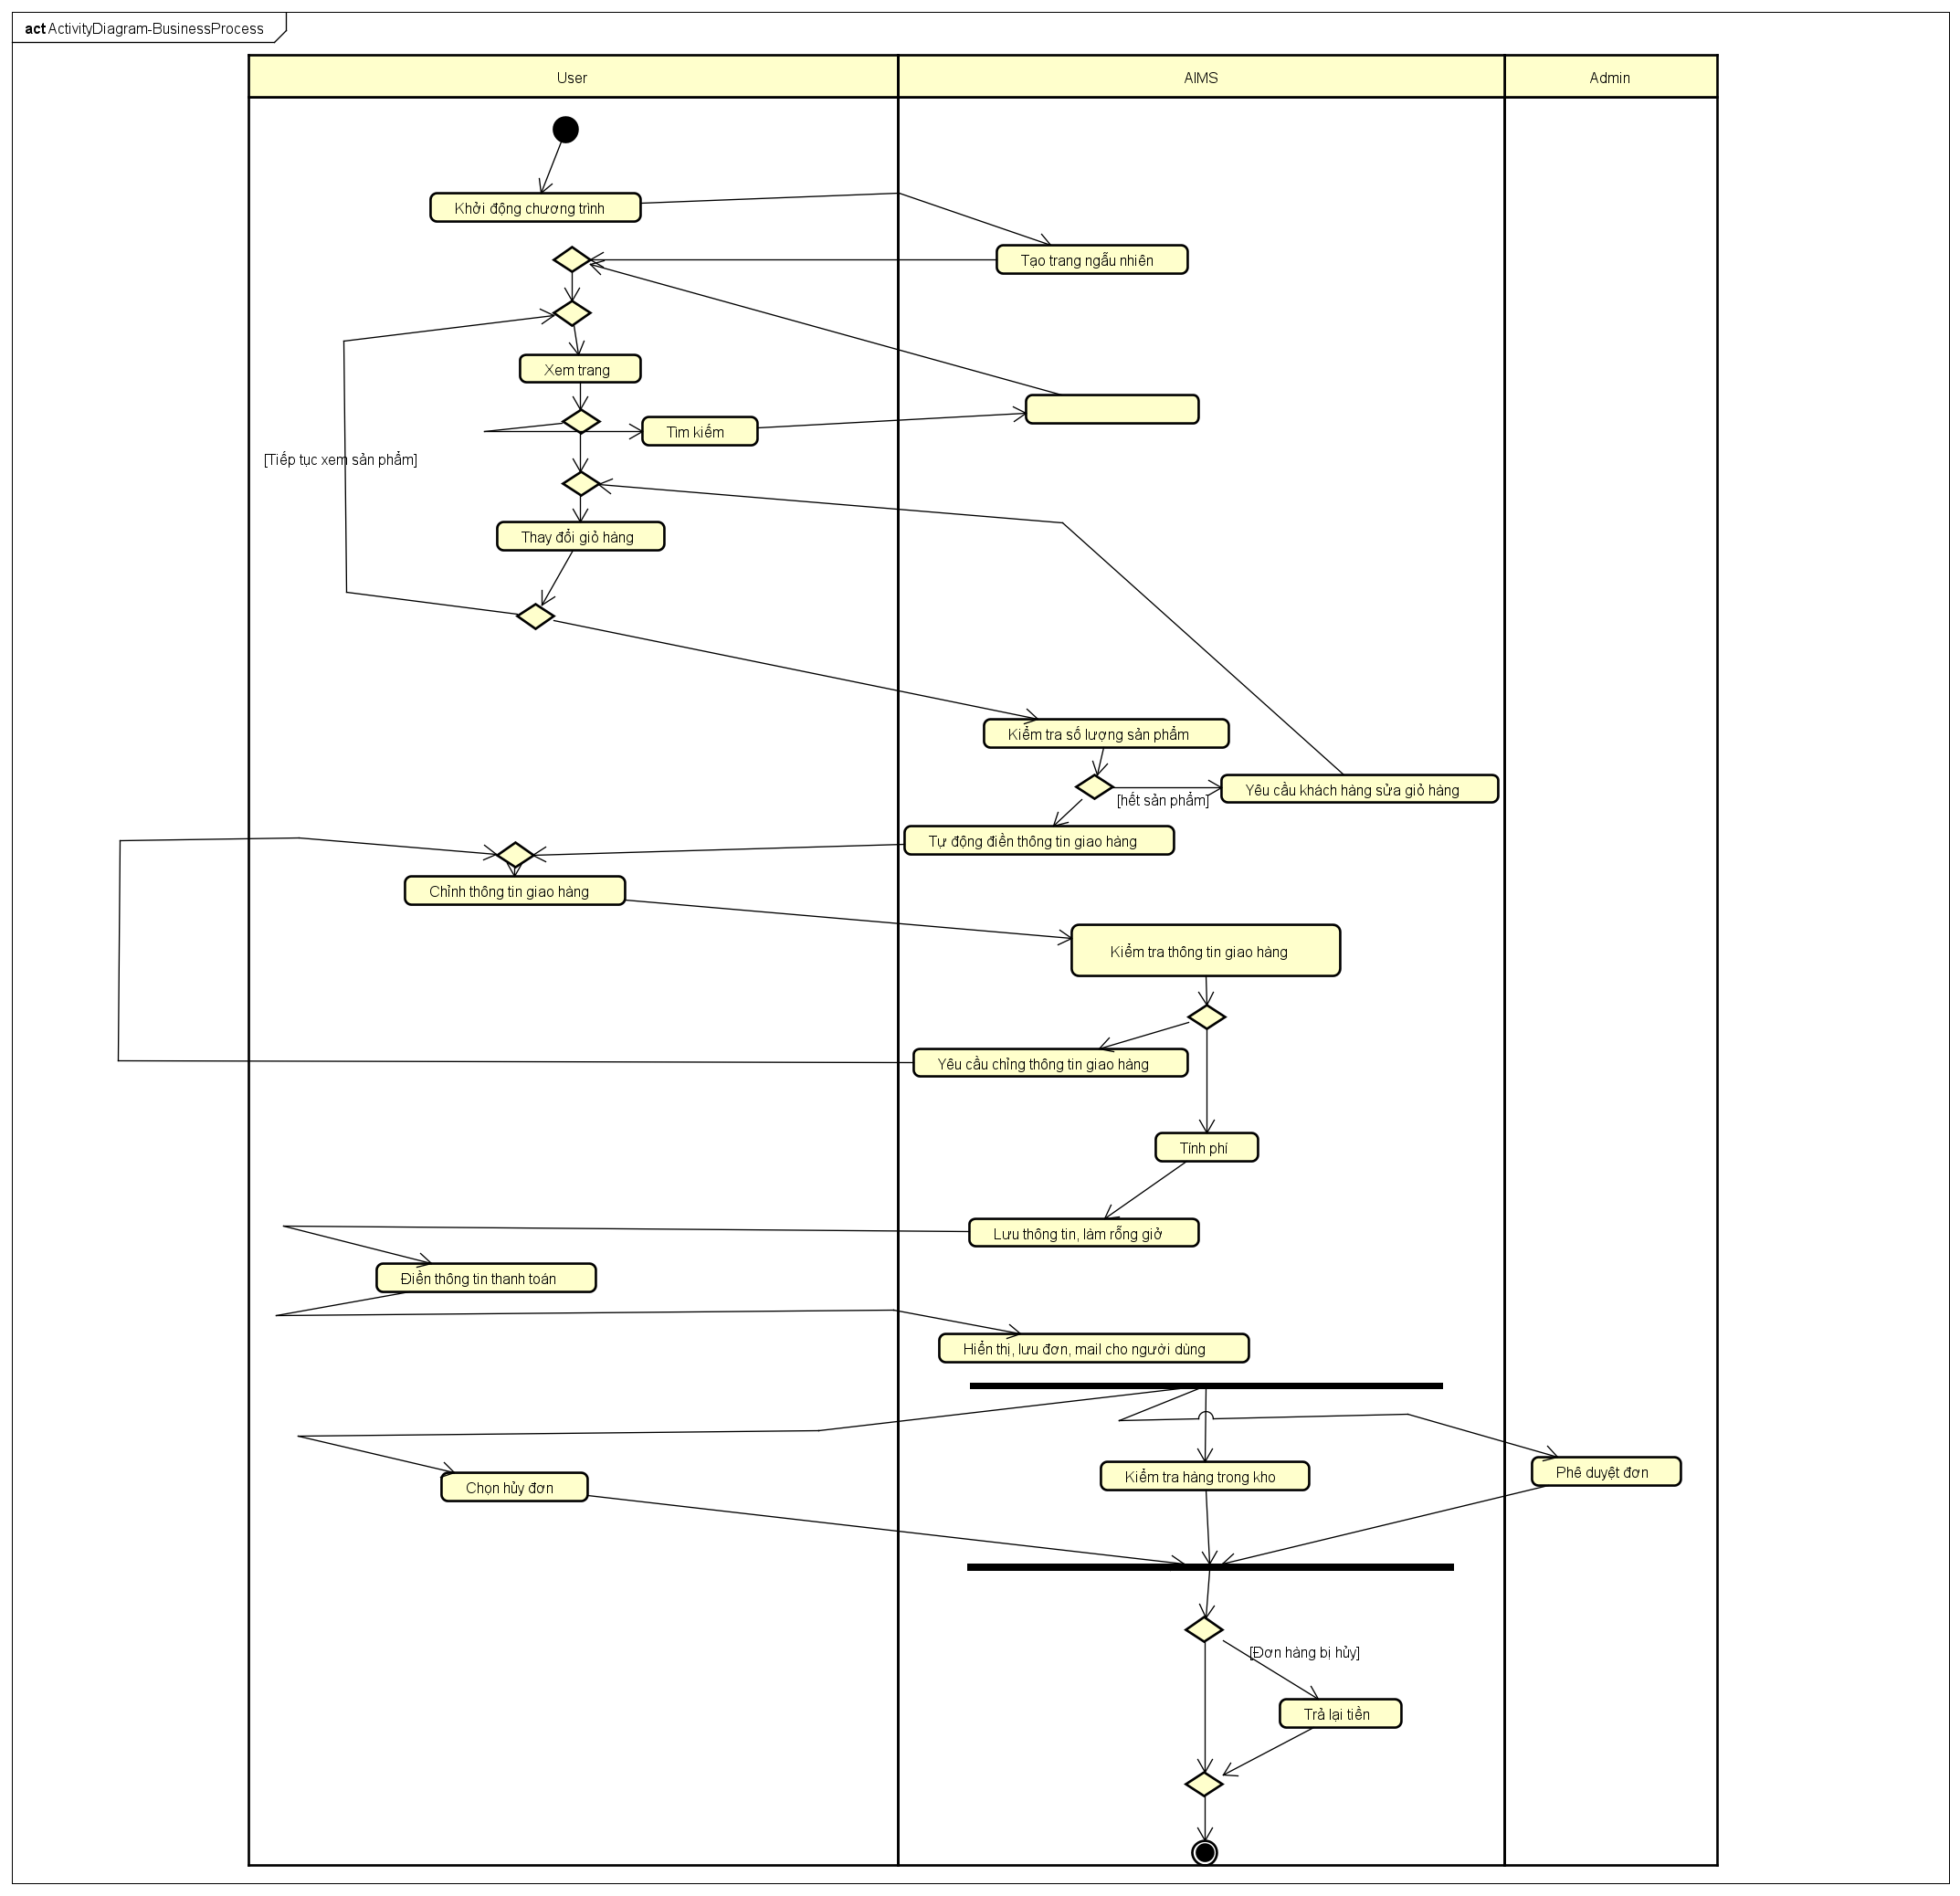
\includegraphics[width=15.24cm,height=16.261cm]{UseCaseDiagram/ActivityDiagram-BusinessProcess.png}

\chapter{Detail requirements}
Details of the use cases given in following sections are specified below.
\bigskip

%%%%%%%%%%%%%%%%%%%%%%%%%%%%%%%%%%%%%%%%%%%%%%%%%%%%%%%%%%%%%%%%%%%%%%%%%%%%%%%%%%%%%%%%%%
\section[Specification of Use case UC001 {}- “Place Order”]{Specification of Use case UC001 - “Place Order”}
\subfile{UseCaseSpecification/UC001-PlaceOrder.tex}

%%%%%%%%%%%%%%%%%%%%%%%%%%%%%%%%%%%%%%%%%%%%%%%%%%%%%%%%%%%%%%%%%%%%%%%%%%%%%%%%%%%%%%%%%%
\section[Specification of Use case UC002 {}- “Pay order”]{Specification of Use case UC002 - “Pay order”}
\subfile{UseCaseSpecification/UC002-PayOrder.tex}

%%%%%%%%%%%%%%%%%%%%%%%%%%%%%%%%%%%%%%%%%%%%%%%%%%%%%%%%%%%%%%%%%%%%%%%%%%%%%%%%%%%%%%%%%%
\section[Specification of Use case UC003 {}- “Place rush order”]{Specification of Use case UC003 - “Place rush order”}
\subfile{UseCaseSpecification/UC003-PlaceRushOrder.tex}


\chapter{Supplementary specification}
\textit{{\textless}Presenting other requirements if necessary, including non-functional requirements such as performance, reliability, usability, and supportability; or other technical requirements such as database system, used technology…{\textgreater}}

\section{Functionality}
 {\textless}List of the functional requirements that are general to many use cases. E.g. Among the flow of events of use case, in all the steps that interacts with the database system, if there are errors in the connection or operation processes, there need to be a corresponding error notifications so that the actor knows that the error is related to the database system rather than the user{\textgreater}

\section{Usability}
 {\textless}Requirements that relate to, or affect, the usability of the software. Examples include ease-of-use requirements or training requirements that specify how readily the software can be used by its actors{\textgreater}

\section{Reliability}
 {\textless}Any requirements concerning the reliability of the software. Quantitative measures such as mean time between failure or defects per thousand lines of code should be stated{\textgreater}

\section{Performance}
 {\textless}The performance characteristics of the software. \ Include specific response times. \ Reference related use cases by name{\textgreater}

\section{Maintainability}
 {\textless}Any requirements that will enhance the supportability or maintainability of the software being built{\textgreater}

\section{Design Constraints}
 {\textless}Any design constraints on the software being built{\textgreater}
\end{document}
